\section{The Simulation}
\label{sec:simulation}

\begin{table*}[!tb]
	\centering
	\begin{tabular}{ll}
		\toprule \midrule
		Parameter & Value \\ \midrule \midrule

		Screen and Camera \\ \midrule
		Screen width & \SI{1}{\meter} \\
		Screen height & \SI{65}{\milli\meter} \\
		Horizontal pixels & 1850 \\
		Screen efficiency & \SI{5000}{photons\per electron}\\
		Camera acceptance & \num{1.5e-5} \\
		Camera MCP Gain & 1442 \\
		Camera quantum efficiency & 0.15 \\

		\midrule
		Accelerated electron beam \\ \midrule
		Emittance \(\left(\epsilon\right)\) & \SI{1e-6}{\meter\radian} \\
		% \(\beta\) & \SI{1}{\meter} \\
		% \(\alpha\) & \SI{0.5}{\radian} \\
		Mean energy \(\left(\bar{E}\right)\) & \SI{1.3}{\giga\electronvolt} \\
		Energy spread \(\left(\sigma_E\right)\) & \SI{0.4}{\giga\electronvolt} \\
		Electrons/bunch \(\left(N_{e^-}\right)\) & \num{1e9} \\
		Background photon density & \SI{3.415e4}{\per\meter\squared} \\
		% Thermal electrons \(N_{e^-_\text{thermal}}\) & \SI{0.016}{\per\second} \\
		\bottomrule
	\end{tabular}
	\caption{
		The expected values for many experimental parameters have been
		calculated.
	}
	\label{tab:expected}
\end{table*}

The simulation of this experiment was split into three parts: the simulation of
the beam, the simulation of the effects of the background and camera, and the
reconstruction of the beam in order to measure the parameters of the beam.

\subsection{The Electron Beam}

% TODO explain LCODE electrons

Given enough computing power and time, the simulation of the beam, from the end
of the plasma cell, passing through two quadrupoles and through a dipole and
hitting the scintillator screen could have been done on
BDSIM~\cite{agapov2009bdsim}, a Geant4~\cite{agostinelli2003geant4} toolkit for
simulating radiation traveling through an accelerator and accelerator
components. This software package simulates the motion of each particle
individually, updating it's position and velocity at each step through the
accelerator by applying forces from the fields of each component of the
accelerator. For beams consisting of \num{\sim e9} particles, tracking each
particle individually as they travel down the beam line would take enormous
amounts of time and available computing power, and, as this simulation was
required to be performed a large number of times, this would have been
impractical for obtaining any reasonable amount of data.

A new program was written, taking advantage of beam matrices to describe the
beam as a whole. The goal of the first part of this program is to simulate the
intensity of the incident beam at each pixel on the screen.

\subsubsection{BDSIM Calibration}

\begin{figure*}[!tb]
	\centering
	\begin{subfigure}[t]{\columnwidth}
		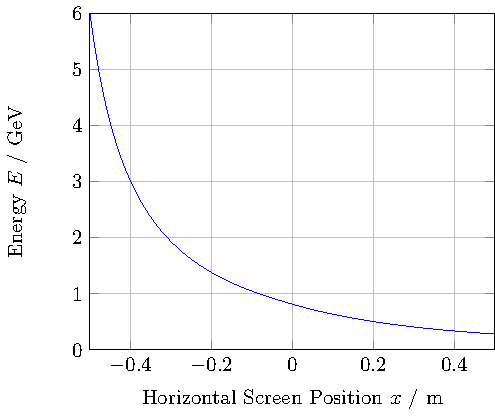
\includegraphics{./figures/eofx.pdf}
		\caption{
			Electron energies corresponding to the horizontal screen position
			due to the effect of the dipole.
		}
		\label{fig:eofx}
	\end{subfigure}\hfill~
	\begin{subfigure}[t]{\columnwidth}
		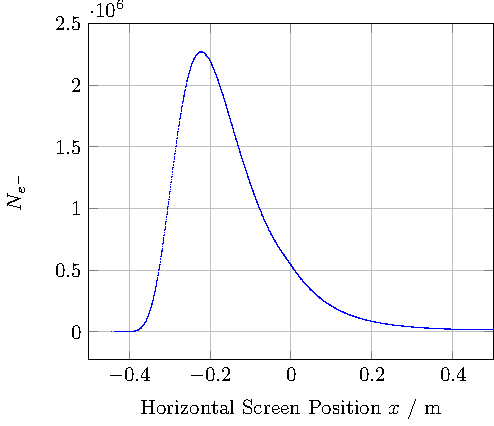
\includegraphics{./figures/edist.pdf}
		\caption{
			The number of electrons expected to hit the screen at each \(x\)
			position for \(E=\SI{1.3}{\giga\electronvolt}\) and
			\(\sigma_E=\SI{0.4}{\giga\electronvolt}\).
		}
		\label{fig:edist}
	\end{subfigure}
	\caption{
		The functions \(E(x)\) and \(N_{e^-}(x)\) extracted from the BDSIM
		calibration output data. These functions are used to calculate the
		horizontal spread of the electrons across the screen.
	}
\end{figure*}

The effect of the quadrupole and the dipole are dependant on the energy of the
individual electrons in the beam.  So to calculate the density and energy of the
electrons as a function of the horizontal screen position a number of BDSIM
simulations were run. \num{1e5} electrons where fired individually down the
simulated AWAKE beam line. These electrons had a square energy distribution from
\SIrange{0}{10} {\tera\electronvolt}, and had a Gaussian spacial distribution
with \(\sigma_x = \sigma_y = \SI{6}{\milli\meter}\) (this is the size of the
iris at the end of the plasma), and no transverse momentum. This large energy
range was chosen to encompass the entire energy range that would hit the screen.
The dipole was set to it's highest setting of \SI{650}{\ampere} to achieve the
maximum spread of the beam on the screen.

% TODO why use no emittance beams for calibration
These BDSIM runs were used to plot the function in Figure~\ref{fig:eofx} which
shows the relationship between an electron's energy and where is it expected to
hit the screen. Figure~\ref{fig:edist} is an example of the horizontal
distribution of a beam of electrons, with a Gaussian energy spread, onto the
screen and all other experimental parameters set to their expected default
value. This was calculated by applying \(x(E)\), the inverse of the function
\(E(x)\) shown in Figure~\ref{fig:eofx}, to the energy distribution of the beam.

At these settings of the experiment, all of the electrons of the beam hit the
screen, allowing for an more accurate measurement of the beam parameters.  The
effect of the emittance and quadrupoles on the horizontal spread is taken to be
negligible in comparison to the effect of the dipole, so it's effect is taken
into account by adding a horizontal smearing to the horizontal position of each
electron on the screen. This means that this plot in Figure~\ref{fig:eofx} is
all that is required to simulate the transverse spread of the beam.

The drift distances from the second quadrupole to the screen were also recorded
for each \(x\) position on the screen. This function \(d(E(x))\) is used in the
calculation of the vertical beam size.


\subsubsection{Deriving the Beam Size Function}

The dipole spreads the beam horizontally across the screen. The electrons in
each vertical strip of pixels are grouped together and their energy approximated
to be equal. This is allowed as the energy spread in each strip will always be
less than \SI{0.5}{\percent}. This was calculated from data used to plot
Figure~\ref{fig:eofx}, by finding the ratio between the difference in energies
between adjacent strips, by the energy value at that strip. This was done for
all strips and the maximum value was a \SI{0.5}{\percent} difference in energy.

Using this assumption, we are able to create one beam and transport matrix for
electrons in each vertical stream of pixels. The root mean square of the
vertical beam size on the screen can be extracted from the resultant beam matrix
\(\bm{\sigma}_1\). To arrive at this beam matrix, the transport matrix
\(\mathcal{M}\) is applied to the initial beam matrix \(\bm{\sigma}_0\) using
(\ref{eq:apply}). The transport matrix is the product of the transport matrices
of each component of the spectrometer:
\begin{equation}
	\begin{split}
		\mathcal{M} = \mathcal{M}_D(d) \cdot \mathcal{M}_{QD}(l_2) \cdot
		\mathcal{M}_D(g_2) \\
		\cdot\;\mathcal{M}_{QF}(l_1) \cdot \mathcal{M}_D(g_1)
	\end{split}
\end{equation}
where \(\mathcal{M}_D\) is the drift transport matrix which is a function of the
travel distance and \(\mathcal{M}_{QF}\) and \(\mathcal{M}_{QD}\) are the
transport matrices of the quadrupole. \(g_1\) is the drift distance (the gap)
between the end of the plasma cell and the first quadrupole, \(g_2\) is the gap
between the two quadrupoles, \(l_1\) and \(l_2\) are the effective quadrupole
lengths of the focusing and defocusing quadrupoles respectively. \(d\) is the
drift distance between the second quadrupole and the screen, taking into account
the effect of the dipole, hence, is a function of the energy which was
calculated in the BDSIM calibration stage.

For simplicity, it is assumed that the quadrupoles strengths \(k_1\) and \(k_2\)
are set to values such that each quadrupole focuses at the mean energy of the
beam, hence these variables are proportional to the beam's mean energy.

% TODO why is the first gap not taken into account? or why it equal zero
% how are the quadrupole lengths calculated?

% The beam matrix element \(\sigma_{11} = \langle y \rangle^2 = \epsilon\beta\)

By applying the matrix multiplication the vertical beam size as a
function of the horizontal screen position can be extracted:
\begin{equation}
	\begin{split}
		\sigma_y^2 = \sigma_{1,11} =\: & C^2(x)\sigma_{0,11} \\
									&+ 2C(x)S(x)\sigma_{0,12} \\
									&+ S^2(x)\sigma_{0,22}
	\end{split}
\end{equation}

Using this beam spread function, a Gaussian distribution of electrons for each
vertical pixel strip is generated with \(\sigma_y^2\) used as the variance of
the distribution.  After generating, a two dimensional histogram representing
the number of electrons hitting the screen at each pixel the goal is to simulate
the effectiveness of the equipment and the effect of background noise then
translate this number to represent the raw signal that will be received from the
camera.

\subsection{Backgrounds}

How good the measurement of the emittance is, is most dependant on the magnitude
of the multiple sources of backgrounds as well as the reliability of the
equipment. The following sources of error were taken into account: the
efficiency of the scintillator screen, the acceptance of the camera due to it's
distance from the scintillator screen, the background photon density, the
emittance of photoelectrons in the camera, the thermal noise in the camera, the
amplification by the microchannel plate (MCP) and the readout noise.  Each
source of noise is added to each pixel independently.

% TODO scintillator cosine distribution

% TODO cite 5000
The first two error sources, arise from the effects of the scintillator screen
and the camera acceptance, both of which scale the original signal. So for each
electron that hits the screen, it is expected that an average of \num{5000}
photons are to be emitted radially with a cosine distribution. The camera
acceptance, is the ratio of photons that the camera registers to the number of
photons emitted by the scintillator, which is expected to be \num{1.5e-5}.
After the addition of these two effects, the camera is expected to receive
\SI{7.5}{\percent} of the original electron signal. The expected value for the
number of photons incident on the camera, is generated using a Poisson random
number with the mean set to the expected value.

It is assumed that there is a uniform distribution of background photons
incident on the camera. The density of these electrons is expected to be
\SI{\sim3.4e4}{photons\per\meter\squared} equating to \num{0.01} background
photons per pixel during the \SI{3e-3}{\second} the gate is open. The number of
background photons that hits a pixel is a discrete value, and so is also
generated using Poisson random numbers.  As discussed later in
Section~\ref{sec:results}, this value is very small in comparison to the signal
produced by the beam and will only have an effect on the measurements if the
density of background photons is multiple magnitudes larger than the expected
value.

 % TODO cite 0.15
The camera's photomultipliers then convert the photons of light back to an
electrical current. This multiplies the incident number of photons by the
quantum efficiency of the camera, \num{0.15}.  The expected number of thermal
photoelectrons per pixel per second is expected to be
\num{0.016}~\cite{istarscmos}, with the camera running at the expected
temperature of \SI{-30}{\celsius} with \SI{16}{\celsius} cooling water and an
ambient room temperature of \SI{16}{\celsius}. Note that this value is typically
doubles for each \SI{5}{\celsius} rise in temperature of the
camera~\cite{istarscmos}.  At these running temperatures of the camera, about 9
photoelectrons are expected to be generated during the time the gate is open,
which is an insignificant proportion in comparison to the beam signal, creating
\num{1e7} photoelectrons before MCP amplification. This effect however is still
simulated asto accomodate for any possible changes to the temperature.

The microchannel plate amplifies the number of photoelectrons by
\num{1442}~\cite{istarscmos}, also amplifying all previously added backgrounds.
This was simulated by scaling the value of the bin, and it's error, by
\num{1442} rather than generating a Poisson random number. The modelling of this
process may not be reflect the true nature of this process due to a lack of
understanding the in underlying process, however the overall effect of scaling
the signal and it's error remains accurately simulated.

And finally, before the values of the signal is obtained, a readout noise is
added. This background is expected to add \num{7.2} readout electrons per image
pixel for the camera operating at \SI{1}{\mega\hertz}~\cite{istarscmos}.
% TODO see camera description for the readout noise

\subsubsection{Error Calculations}

Poisson statistics were used for the calculation of errors.  Once the shape of
the incident beam on the screen was calculated the number of electrons incident
on each pixel was given an error of the square root of the count. Two methods of
error propagation were used depending on the nature of the process involved.
The following processes were modeled as additive processes: background photons
hitting the screen, the thermal electrons from the currents in the camera and
the readout noise, whereas the following were modelled as multiplicative
processes: photon generation at the scintillator screen, photoelectron
generation in the camera PMTs and the amplification of the electron signal by
the MCP.

Basic error propagation techniques were used here. For the additive processes,
where the new value of each bin $n$ is the sum between the old bin value $n_0$
and the value given by the process $n_\text{proc}$: $n=n_0+n_\text{proc}$ the
propagation of error is given by calculating the hypotenuse of the absolute
errors:
\begin{equation}
	\Delta n= \sqrt{\Delta n_0^2 + \Delta n_\text{proc}^2}
	\label{eq:error_add}
\end{equation}
where the error of a Poisson random number is the square root of the value.

For the multiplicative processes, i.e. $n = \lambda_\text{proc}n_0$, where
$\lambda_\text{proc}$ is the scaling factor of the process the propagation of
the error is given by calculating the hypotenuse of the percentage errors:
\begin{equation}
	\Delta n= n \sqrt{
		\left( \frac{\Delta n_0}{n_0} \right)^2 +
		\left( \frac{\Delta \lambda_\text{proc}}{\lambda_\text{proc}} \right)^2}
	\label{eq:error_mul}
\end{equation}

Many of the errors \(\Delta n_\text{proc}\) and \(\Delta \lambda_\text{proc}\)
were unavailable at the time of simulation. All background noises are modeled as
uniformly distributed Poisson random numbers so under these assumptions the
associated error on each value can correctly be taken to be the square root of
the value. % TODO you sure not the sqrt of the mean value?
So for missing \(\Delta n_\text{proc}\) values, (\ref{eq:error_add}) becomes
\begin{equation}
	\Delta n= \sqrt{\Delta n_0^2 + \sqrt{n}^2} = \sqrt{\Delta n_0^2 + n}
\end{equation}
and for multiplicative processes, the resultant values were also Poisson random
numbers meaning (\ref{eq:error_mul}) can be rewritten as
\begin{equation}
	\begin{split}
		\Delta n &=
		n \sqrt{
			\left( \frac{\Delta n_0}{n_0} \right)^2 +
			\left( \frac{\sqrt{n}}{n} \right)^2
		} \\[1em]
		&= n \sqrt{
			\left( \frac{\Delta n_0}{n_0} \right)^2 +
			\frac{1}{n}
		}
	\end{split}
\end{equation}
where the full statistical error of the generated value is taken into account
without knowledge of the error of the scaling factor.
% TODO simply scaling the errors up with the MCP?

\subsection{Calculating the Emittance}

The signal received from the camera is required to be scaled back to represent
the real beam size on the screen. The effect of additive backgrounds and scaling
processes are reverted in the reverse order of their application arriving at a
measured value for the number of electrons that hit the screen at each pixel.

To calculate the vertical beam size for each pixel strip, a Gaussian function is
fitted to the vertical beam profile using CERN ROOT's \(\chi^2\) minimising
fitting algorithm~\cite{Brun:1997pa}.
% TODO gaussian function
The root mean square of the fitted
Gaussian is then calculated for each strip to obtain the vertical beam size at
each horizontal position on the screen. These points are displayed as the black
points in the beam reconstruction plots in Figures~\ref{fig:default}
and~\ref{fig:yoverestimate}.

Finally, the vertical beam size function, displayed as the black line in the
beam reconstruction plots and which was previously used to simulate the shape of
the incident electron beam, is then fitted to the measured beam sizes. Again,
the fitting is done wholly using ROOT's \(\chi^2\) minimising fitting algorithm,
where the three beam parameters \(\epsilon\), \(\beta\) and \(\gamma\) as
parameters to be minimised.

